%%%%%%%%%%%%%%%%%%%%%%%%%%%%%%%%%%%%%%%%%%%%%%%%%%%%%%%%%%%%%%%%%%%%%%%%%%%%
% AGUJournalTemplate.tex: this template file is for articles formatted with LaTeX
%
% This file includes commands and instructions
% given in the order necessary to produce a final output that will
% satisfy AGU requirements, including customized APA reference formatting.
%
% You may copy this file and give it your
% article name, and enter your text.
%
%
% Step 1: Set the \documentclass
%
%

%% To submit your paper:
\documentclass[draft]{agujournal2019}
\usepackage{url} %this package should fix any errors with URLs in refs.
\usepackage{lineno}
\usepackage[inline]{trackchanges} %for better track changes. finalnew option will compile document with changes incorporated.
\usepackage{soul}
\linenumbers
%%%%%%%
% As of 2018 we recommend use of the TrackChanges package to mark revisions.
% The trackchanges package adds five new LaTeX commands:
%
%  \note[editor]{The note}
%  \annote[editor]{Text to annotate}{The note}
%  \add[editor]{Text to add}
%  \remove[editor]{Text to remove}
%  \change[editor]{Text to remove}{Text to add}
%
% complete documentation is here: http://trackchanges.sourceforge.net/
%%%%%%%

%\draftfalse

%% Enter journal name below.
%% Choose from this list of Journals:
%
% JGR: Atmospheres
% JGR: Biogeosciences
% JGR: Earth Surface
% JGR: Oceans
% JGR: Planets
% JGR: Solid Earth
% JGR: Space Physics
% Global Biogeochemical Cycles
% Geophysical Research Letters
% Paleoceanography and Paleoclimatology
% Radio Science
% Reviews of Geophysics
% Tectonics
% Space Weather
% Water Resources Research
% Geochemistry, Geophysics, Geosystems
% Journal of Advances in Modeling Earth Systems (JAMES)
% Earth's Future
% Earth and Space Science
% Geohealth
%
% ie, \journalname{Water Resources Research}


% 12 Publication Units (500 words or one figure)
% 1 Table: list of distributions
% 2 Image: illustration of orientation
% 3 Image (appendix): multi-panel comparison of performance
% 4 Image distributions (filtered, sheltered/unsheltered)
% 5 image standard deviation and wind


\journalname{JGR: Atmospheres}


\begin{document}

\title{Observation of falling snow orientation in sheltered and unsheltered observation sites}


\authors{J. Grazioli\affil{1}, M. Condolf\affil{2}, F. Coletti\affil{2}, and A. Berne\affil{1}  }


\affiliation{1}{Environmental Remote Sensing Laboratory, École Polytechnique Fédérale de Lausanne, Lausanne, Switzerland}
\affiliation{2}{Department of Mechanical and Process Engineering, ETH, Zürich, Switzerland}
% \affiliation{3}{Third Affiliation}

\correspondingauthor{Jacopo Grazioli}{jacopo.grazioli@epfl.ch}

%% Keypoints, final entry on title page.

%  List up to three key points (at least one is required)
%  Key Points summarize the main points and conclusions of the article
%  Each must be 140 characters or fewer with no special characters or punctuation and must be complete sentences

\begin{keypoints}
\item Observations of falling snowflake orientations show symmetrical distributions around 0°, aligning with some previous literature assumptions.
\item Sheltered and unsheltered sites show differences in orientation distributions, influenced by wind. Instrument (local perturbations) and atmospheric effects cannot be separated.
\item Numerical simulations reveal previously reported non-zero median orientations as artifacts, identifying better estimation methods.
\end{keypoints}



\begin{abstract}
This study investigates the orientation of falling snowflakes using data from a Multi-Angle Snowflake Camera (MASC). We explore the impact of different observational setups (sheltered vs. unsheltered), wind conditions, hydrometeor type, and axis ratio on the orientation distributions. Numerical simulations are used to select the best orientation estimator and to understand the reason behind different results reported in past literature. We find that previously reported non-zero median orientations are likely artifacts of averaging absolute values from individual cameras. Observed orientations generally follow a symmetrical distribution around 0$^\circ$, with broader and flatter distributions observed in unsheltered sites and high wind conditions.  Observed distributions may vary significantly from those assumed in previous studies, highlighting the need for further research on snowflake orientation under varying environmental conditions.
\end{abstract}

\section*{Plain Language Summary}
Understanding the orientation of falling snowflakes is important for interpreting weather radar data and better understand snowfall micro-physics. This study uses a 3-view camera to capture detailed images of falling snowflakes and estimate their orientations. Snowflakes generally fall with their largest dimension parallel to the ground (horizontal orientation), with variations in both directions around this setup. We found that observations in sites exposed to the wind show broader distributions of orientations compared to those in sheltered areas. Additionally, our simulations suggest that some previous studies may have incorrectly reported average orientations because of the way data was processed. These findings help refine our knowledge of snowflake behavior and show the need of better understanding the physical mechanisms affecting the distribution of snowflake orientations.



\section{Introduction}
Ice-phase hydrometeors, individual crystals and aggregates fall with a preferred orientation; In stable conditions, they align in a way that maximizes the area projected in the direction of flow~\cite{Koebschall_EF_2023}. This fact is exploited by dual-polarization weather radars to retrieve information about the microphysical processes occurring in precipitation and to identify which type of hydrometeors are present and where. Except for relatively rare situations, like storm electrification~\cite<e.g.,>{Krehbiel_MAP_1996,Pineda_JGRA_2019}, the interpretation of radar meteorology rely on the assumption that anisotropic ice particles tend to fall with their major dimension oriented horizontally.
The concept of orientation is thus linked to the anisotropic nature of most hydrometeors and it loses any meaning for isotropic, spherical particles. 

Considering a population of hydrometeors rather than individual particles, as it is often the case for practical applications, the distribution of orientations is often modeled with a relatively narrow variability around 0$^\circ$ (i.e., horizontally oriented) values. Looking at the overview of Table~\ref{table:orientations}, one can observe that modeling studies mostly employ a Gaussian distribution, with standard deviations varying between 3$^\circ$~\cite<e.g.>{Matrosov_JAM_2001} and 60$^\circ$~\cite<e.g.>{Putnam_MWR_2017} depending on the type of hydrometeors.  
Observational studies~\cite<as in>{Garrett_GRL_2015} confirmed that there are differences due to hydrometeor type but also due to the environmental conditions (wind and turbulence). Observational studies report non-zero mean and median orientation values, which is contradictory with what stated so far. As we will discuss later in this manuscript, this discrepancy is in reality the result of the way multi-view instrumental observations are combined to retrieve an individual estimate of orientation. 

The problem of observing hydrometeor orientations while they fall, without generating disturbance induced by the measurement itself, is not trivial. Among the ground-based instruments able in principle to perform this task we may cite: the two-dimentional video disdrometer~\cite<2DVD>{Kruger_JAOT_2002}, the multi-angle snowflake camera~\cite<MASC>{Garrett_AMT_2012}, the Precipitation Imaging Package~\cite<PIP>{Pettersen_atmosphere_2020} and the latest Video In Situ Snowfall Sensor~\cite<VISSS>{Maahn_AMT_2024}. All relatively recent, they differ for example for the number of simultaneous viewpoints (one for PIP, three for MASC, two for the others), resolution (order of magnitudes of tens of $\mu{m}$ for MASC and VISSS and hundreds of $\mu{m}$ for 2-DVD and PIP) or instrumental structure (compact for MASC and 2-DVD and open for PIP and VISSS). These sensors allow for direct investigations, based on the pictures of individual hydrometeors. As mentioned above, indirect retrievals  of the behaviour of large populations of particles within the sampling volume of remote-sensing instruments are also commonly employed, mostly by means of dual-polarization technologies~\cite<e.g.,>{Matrosov_JAS_2005},

In this manuscript we present an analysis of fall orientation of ice-phase hydrometeors, conducted on a large dataset collected by a MASC. We explore the effect of different siting of the instrument (sheltered or unsheltered), wind conditions, hydrometeor type and axis ratio as well as the estimator of orientation used. For the last investigation, We complement the analysis with simulations aimed at uncovering biases that may emerge with some estimation choices.
 
\section{Data and Methods}
We use a large dataset of MASC data which includes co-located environmental information, notably  temperature, humidity, wind, from the MASCdb database described in~\cite{Grazioli_SD_2022}. The database currently includes about one million of image triplets (e.g. Fig.~\ref{fig:triplet}) and pre-computed geometrical and microphysical descriptors. In this study, we filter the initial database to: (i) remove precipitation falling at positive temperatures, as we focus on dry snow; (ii) we remove particles classified as \textit{small particles} according to the classification of~\cite{Praz_AMT_2017} as their size is too close to the resolution of the images  (about 35$\mu$m); (iii) we remove all the measurements possibly due to wind-blown snow according to~\cite{Schaer_TC_2020}. All the filtering steps are conducted on data already integrated in MASCdb, thus readily reproducible. The filtered dataset includes 412'150 particles. 

While operating with three 2D images of and individual 3D object, the first issue is to obtain one estimate of orientation to assign the the object/snowflake. As snowflakes are often modeled as ellipsoids or spheroids, previous studies on the MASC used the orientation of the major axis of the best-fitting ellipsoid as a proxy for orientation in individual 2D images~\cite{Garrett_GRL_2015,Gergely_JGRA_2016, Fitch_AMT_2021, Fitch_JGR_2022}, and then taking the mean of the absolute value of the three estimates. We refer to this approach to \textit{Mean\_Abs}. Other studies perform instead a 3D reconstruction of an ellipsoid that best fits the three views, and take as estimate the orientation of the major axis of such ellipsoid~\cite{Jiang_JAS_2019}. We refer to this family of approaches as \textit{Ellipsoid\_Fit}. At a first glance in Table~\ref{table:orientations}, the results of the experimental studies using those estimators seem to disprove the common assumption that the distribution of orientations of snowflakes is centered at 0$^\circ$, and modal values between 10$^\circ$ and 20$^\circ$ are reported. While for the \textit{Ellipsoid\_Fit} in ~\cite{Jiang_JAS_2019} this is based on a small sample of aggregates, thus difficult to evaluate, we would like to show that the appearance of non-zero modal values in the \textit{Mean\_Abs} approach is a bias induced by conducting this type of averaging.

To do so, and to select an appropriate estimator of orientation, we conducted numerical simulations (results shown in Fig.~\ref{fig:simulations}). Ellipsoid of randomly varying geometry as well as simulated aggregates and monomers are generated~\cite<as for example in>{Leinonen_AMT_2021} and their projection into MASC-like images is computed in order to test various estimation methods. The orientation of the reference snowflakes or ellipsoid is individually known and it is drawn by a zero-mean and 25$^\circ$ standard deviation from a Gaussian distribution. While this simulation setup has the potential to be exploited much further than this with the variations of all the parameters involved, the goal is here to support the selection of the estimator that we will employ in the actual field-collected data. Figure~\ref{fig:simulations} allows us to have an overview of how well various methods reproduce the distribution of orientation (panel a,c) and the magnitude of the errors with respect to the absolute value of the orientation (panel b, d). We tested the following estimator: \textit{Min}, being the minimum (absolute value) orientation among the views with sign preserved, \textit{Mean\_Abs} as defined above, \textit{Ellipsoid\_fit} as described above, \textit{Mean} being the mean of the estimate of three views, as well as the individual estimates of each view \textit{Cam0}, \textit{Cam1}, \textit{Cam2}. 

The results of this experiment shows first of all that the non-zero modal values of \textit{Mean\_Abs} appear also in this case, thus confirming the hypothesis that this is an artefact of averaging absolute-values, which makes near-zero estimates much less likely to occur. \textit{Ellipsoid\_fit} has small errors, but the modal values of the distribution of this method consistently show a positive bias of a few degrees, such that the reconstructed distribution is not centered exactly at 0$^\circ$. Individual camera views have larger errors as well as very broad reconstructed distributions, a result in itself interesting and worth investigating further as many snowflake imagers have only one view. \textit{Min} provides low errors, but it produces distributions that are exaggeratedly leptokurtic. Therefore in the following, we will use a simple \textit{Mean}, which is an optimal compromise between preserving as much as possible the shape of the distribution with limited errors and extreme simplicity. For this specific experimental setup, \textit{Mean} is also the only method that likely preserves Gaussianity, according to a Kolmogorov-Smirnov test.  

\section{Experimental results and discussion}
The distribution of all the (\textit{Mean}) orientation values presented in Fig.~\ref{fig:alldata} shows that the overall distribution is symmetrical with a mode at 0$^\circ$. The distribution of all observations is fat-tailed. Different type of instrument installations have a clear impact on the distribution: installations within DFIRs, with enhanced wind sheltering and protection from local turbulence shows less pronounced tails while not sheltered sites more pronounced ones as well as a much flatter distribution in the proximity of 0$^\circ$ orientation values, between -25$^\circ$ and 25$^\circ$. It can be hypothesized that this change in shape of the distribution is the result of the different siting, with the unsheltered observations perturbed by \textit{local} turbulence driven by the instrument itself~\cite<as described by>{Fitch_AMT_2021}. 

It is however reasonable to assume that the \textit{atmospheric} conditions should play a role in shaping the distribution of orientation values, with broader distribution in case of strong winds and wind variations. In Fig.~\ref{fig:wind-effect} we compare the evolution of the standard deviation of orientation distributions for DFIR and unsheltered conditions at various levels of horizontal winds. At low winds ($<1$ms$^{-1}$), the curves are relatively close, as well as for high winds ($>10$ms$^{-1}$) while they depart up to 5/6$^\circ$ for intermediate conditions, with the DFIR curve increasing as the wind increases. It can be assumed that for near-zero winds local turbulence due to the instrument itself is minimal, and sheltered and unsheltered conditions are substantially equivalent. It is however not straightforward to interpret the behaviour of the curves in case of stronger winds. One explanation could be that as the wind gets stronger, the DFIR shelter gets less effective, leading to a broadening of the distribution (broadening due to local interactions with the instrument). However, strong wind conditions could broaden the distribution as well (broadening due to atmospheric causes) and a combination of the two mechanisms is plausible. Further research would be needed to clarify this aspect and for the time we can simply report this discrepancy among the different siting types. 

Under the assumption that measurements collected within a DFIR are inherently less perturbed, we focus now the attention only on this type of siting. Given the large size of the original dataset, we can perform further data stratification. Figure~\ref{fig:hydroclass} shows the distribution of orientations in two contrasting wind regimes ($<4$ms$^{-1}$ and $>8$ms$^{-1}$), stratified according to hydrometeor type~\cite<method of>{Praz_AMT_2017} and average axis ratio of the particles (divided in two classes of below- and above-median axis ratio).  The effect of stronger winds results in broader and platykurtic distributions, which lose the clear median around 0$^\circ$ orientation values. For columnar and planar crystals of elongated shape (low axis ratio), this results in distributions that start to exhibit off-zero modal values, that are not observed in low-wind conditions. 
The effect of axis ratio on the distribution is not remarkable, but this is an important information in itself: we can exclude that the modal values around 0$^\circ$ may be artefacts resulting from near-spherical axis-symmetrical particles being assigned a quasi-horizontal orientations merely because of geometrical conventions. 

If we focus only on low-wind conditions ($<4$ms$^{-1}$) within DFIR sites, a situation that should minimize perturbations for our dataset, the distribution of orientation values has $\sigma$ of 28$^\circ$ (graupel), 30$^\circ$ (aggregates), 32$^\circ$ (planar crystals), and 34$^\circ$ (columnar crystals), 29.5$^\circ$ (all mixed). Those values are within the range of commonly assumed ones, as reported in Table~\ref{table:orientations}, but depart significantly from individual studies especially the ones assuming extremely narrow distributions~\cite{Matrosov_JAM_2001,Matrosov_JAS_2005}, or the ones assuming much broader distributions~\cite<e.g.>{Ryzhkov_JAMC_2011, Bukovic_JAMC_2018}. Further research on the actual distribution of orientations is needed to fine-tune those estimates, especially in order to understand the effect of actual atmospheric conditions, not instrument-induced, on distribution shape and breadth. 

\section{Conclusions}
The main results of this letter devoted to the estimation of the orientation of falling snowflakes with a MASC are:
\begin{itemize}
    \item Estimation of orientation as the mean of the orientation of the best fit ellipsoid of each camera views is a good compromise in terms of error minimization and correct reproduction of the distribution of orientation values. 
    \item Previous studies reporting median orientations departing from 0$^\circ$ are most likely resulting from artefacts due to averaging the \textit{absolute value} of the orientation of each camera view.
    \item Single-camera estimates are largely more uncertain than a combination of the three views.
    \item Field measurements on a large dataset show that orientation values have overall a symmetrical distribution around 0$^\circ$.
    \item Observations collected in unsheltered sites as well as in sheltered sites in strong wind conditions result in broader and flatter distributions, with a less clear mode at 0$^\circ$. This is probably both an artefact of local disturbances (instrument-induced) as well as actual environmental phenomenon. It is not possible in this set-up to separate the two effects and further research is needed in this field.
    \item Observed orientation distributions can differ largely with respect to assumptions made in previous studies. 
\end{itemize}

% ---------------
 \begin{table}
 \caption{Non-exhaustive list of research works that provide assumptions or measurements of the distribution of orientation angles of ice phase particles. $\overline{\theta}$ indicates mean orientation, $\sigma$ is the standard deviation,  $\theta_{M}$ indicates the mode of the distribution, $\theta_{Q50}$ is the median, $MAD(\theta)$ is the median absolute deviation.}
 \label{table:orientations}
 \centering
 \begin{tabular}{l p{80mm}} 
 \hline
  Ref.   & Details \\
 \hline
   \cite{Matrosov_JAM_2001} & $\overline{\theta} = 0^\circ, \sigma = 3^\circ$ \\
   \hline
   \cite{Matrosov_JAS_2005} & $\overline{\theta} = 0^\circ, \sigma = 9^\circ \pm3^\circ$ (dendrites) \\
   \hline
    \cite{Kennedy_JAMC_2011}  &   $\overline{\theta} = 0^\circ, \sigma = 15^\circ$ (dendrites) \newline $\overline{\theta} = 0^\circ, \sigma = 30^\circ$ (aggregates)     \\
   \hline
    \cite{Ryzhkov_JAMC_2011} & $\overline{\theta} = 0^\circ, \sigma = 40^\circ$ (aggregates) \newline 
   $\overline{\theta} = 0^\circ \sigma = 40^\circ$ (graupel) \\
   \hline
   \cite{Hogan_JAMC_2012} & Assumed horizontal  \\
   \hline   
   \cite{Putnam_MWR_2017} & $\overline{\theta} = 0^\circ \sigma = 20^\circ$ (snow) \newline 
   $\overline{\theta} = 0^\circ \sigma \in [0,60]^\circ$ (graupel) \\
   \hline
   \cite{Bukovic_JAMC_2018} &  $\overline{\theta} = 0^\circ, \sigma = 10^\circ$ (dendrites) \newline  $\overline{\theta} = 0^\circ \sigma = 40^\circ$ (aggregates) \\
   \hline
    \cite{Matsui_JGRA_2019}  & $\overline{\theta} = 0^\circ \sigma = 20^\circ$ (aggregates) \newline 
   $\overline{\theta} = 20^\circ \sigma = 42^\circ$ (graupel) \\
   \hline
   \cite{Garrett_GRL_2015}$^*$ & $\theta_{Q50} = 39^\circ, \theta_{M} = 13^\circ$ (aggregates) \newline
   $\theta_{Q50} = 35^\circ, \theta_{M} = 16^\circ$ (rimed particles) \newline
   $\theta_{Q50} = 35^\circ, \theta_{M} = 20^\circ$ (graupel) \newline
   $\theta_{Q50} = 28^\circ, \theta_{M} = 13^\circ$ (low-turbulence, all types) \newline
   $\theta_{Q50}= 40^\circ, \theta_{M} = 23^\circ$ (high-turbulence, all types) \\
   \hline
   \cite{Gergely_JGRA_2016}$^*$ &  $\theta_{Q50} \in [38,47.3]^\circ$, $MAD(\theta) \in [43,51]^\circ$ \\
   \hline
   \cite{Jiang_JAS_2019}$^*$ & $\theta_{M}\approx 10^\circ$ \\
   \hline
   \cite{Fitch_AMT_2021}$^*$ & $\theta_{M} = 57^\circ$ (wind $> 5$ ms$^{-1}$) \newline
   $\theta_{M} = 28^\circ$ (wind $< 1.5$ ms$^{-1}$) \\
   \hline
   \cite{Fitch_JGR_2022}$^*$ & $\theta_{M} = 3^\circ$ 
   \newline
   $\theta_{M} = 13^\circ$ (different estimations)  \\
   \hline
   \cite{Schrom_JAS_2023}$^*$ & Beta distribution (varying parameters) \\
   \hline
    \multicolumn{2}{l}{$^{*}$Papers that present orientation statistics from ground-based measurements.}
 \end{tabular}
 \end{table}


% Giving latex a width will help it to scale the figure properly. A simple trick is to use \textwidth. Try this if large figures run off the side of the page.
\begin{figure}
 \noindent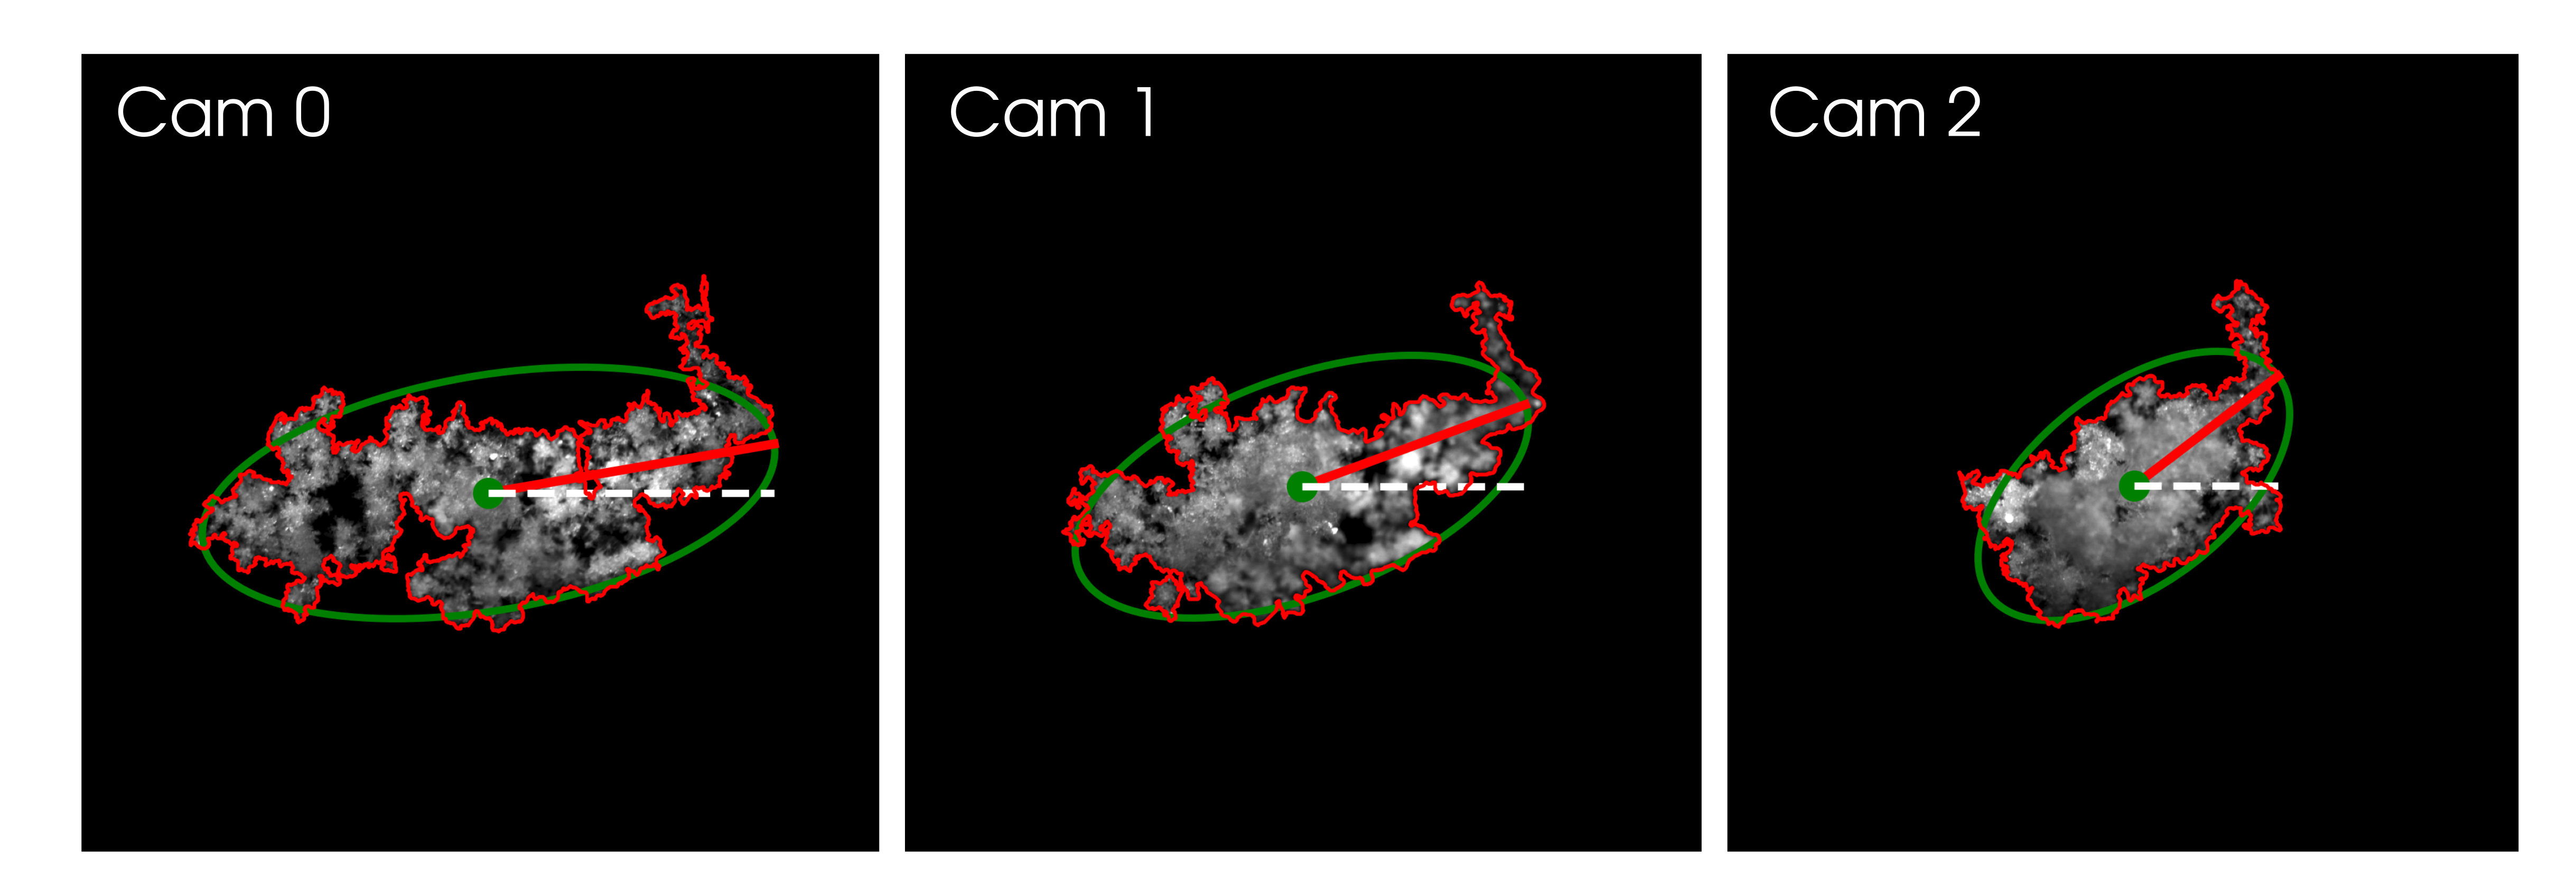
\includegraphics[width=\textwidth]{Fig01.png}
\caption{Example of a triplet of images of a snow aggregate, collected by a MASC. The best fitted ellipse of each image is drawn in green, with the major axis defining the apparent orientation with respect to the horizontal.    }
\label{fig:triplet}
\end{figure}


\begin{figure}
 \noindent \centering \includegraphics[width=\textwidth]{Fig02.png}
\caption{Evaluation of the retrieval of orientation that could be achieved with a triplet of MASC images, conducted using simulated data (ellipsoids in the left column, simulated snowflakes in the right column). (a) and (c): distribution of orientation value, both reference and reconstructed. (b) and (d): letter-value plots of the distribution of the error of the estimation of the absolute value of the orientation. The simulations are conducted on 10'000 ellipsoids of various geometry as well as on 10'000 aggregates. }
\label{fig:simulations}
\end{figure}

\begin{figure}
 \noindent \centering 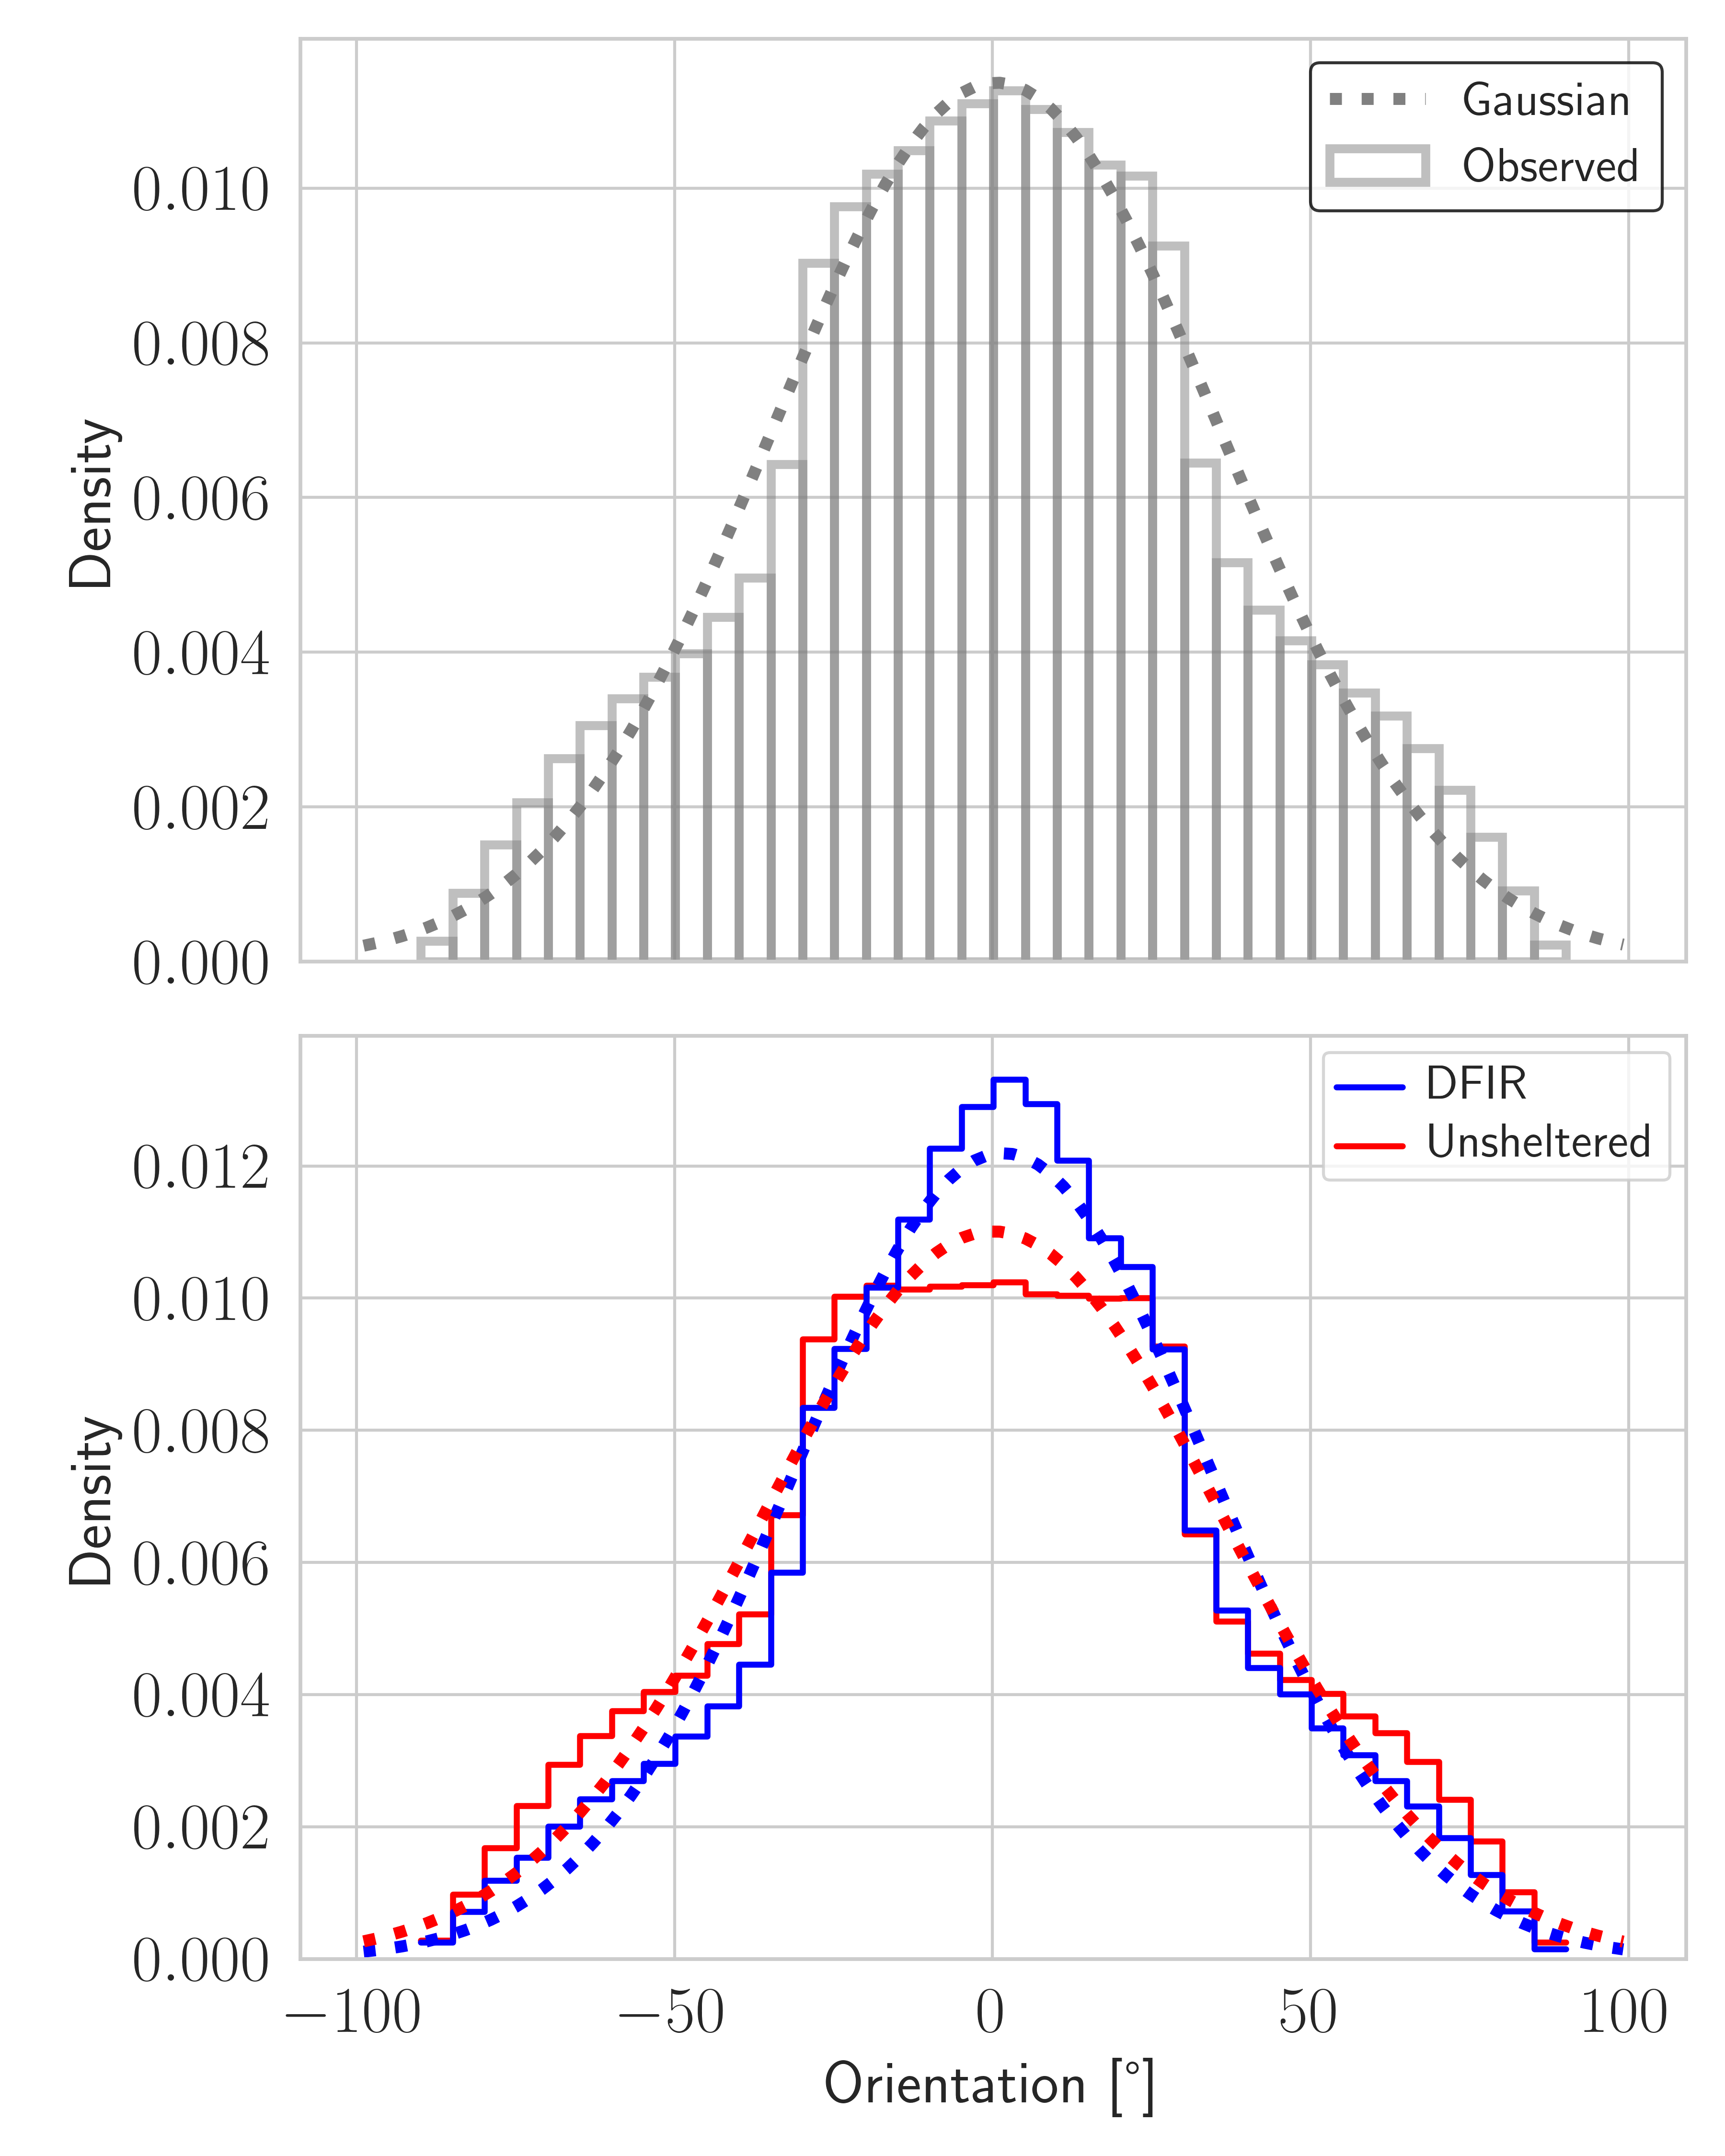
\includegraphics[width=\textwidth]{Fig03.png}
\caption{Histogram of the distribution of orientation value for all data (412'150 particles, top) and data stratified according to the instrumental setup (bottom) either being unsheltered (274'839 particles) or deployed within a double-fence inter-comparison reference (DFIR, 137'311 particles). The dotted lines illustrate the shape of a Gaussian curve having the same mean and standard deviation as the observed data, and are given to provide a visual comparison of the difference with respect to a Gaussian shape (it is not a fit of the histogram). Orientation values are estimated as the sign-preserving mean of the three MASC views.   }
\label{fig:alldata}
\end{figure}
 
\begin{figure}
 \noindent \centering 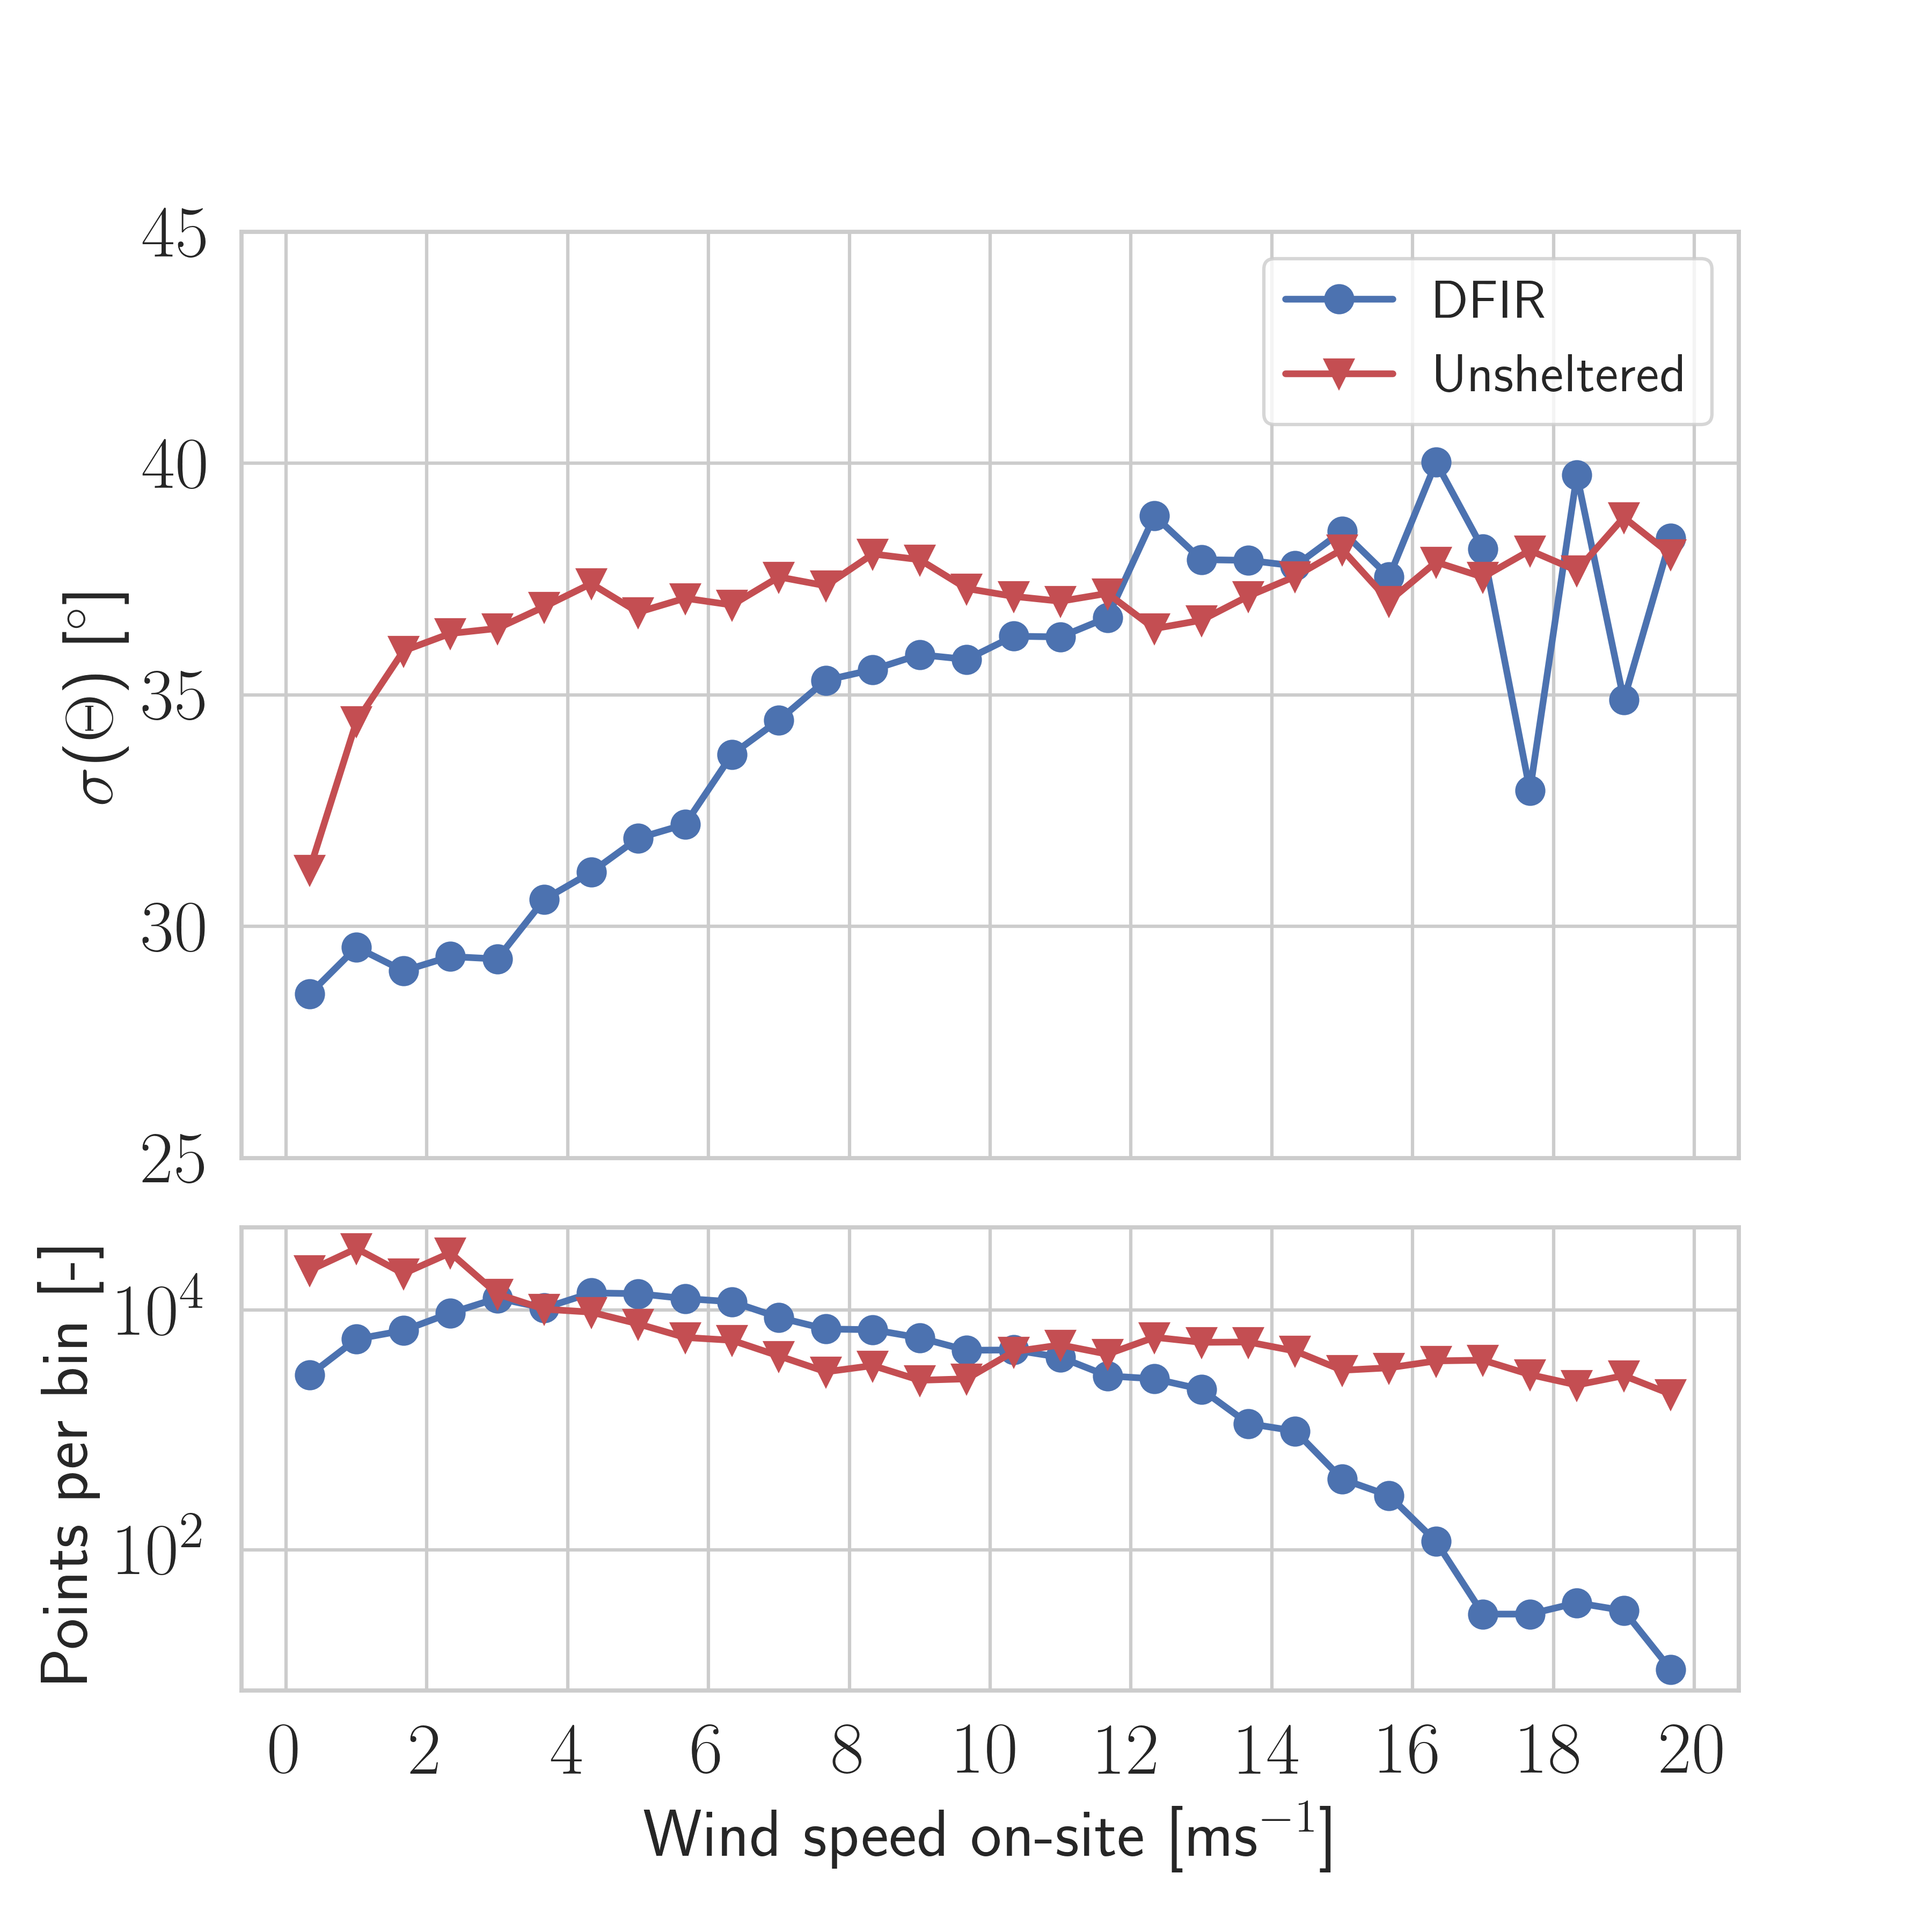
\includegraphics[width=\textwidth]{Fig04.png}
\caption{Evolution of the standard deviation of the  distribution of orientation values at various wind speed levels and stratified according to the instrumental setup. The bottom panel shows the number of observations falling into each bin of wind speed.  }
\label{fig:wind-effect}
\end{figure}

\begin{figure}
 \noindent \centering 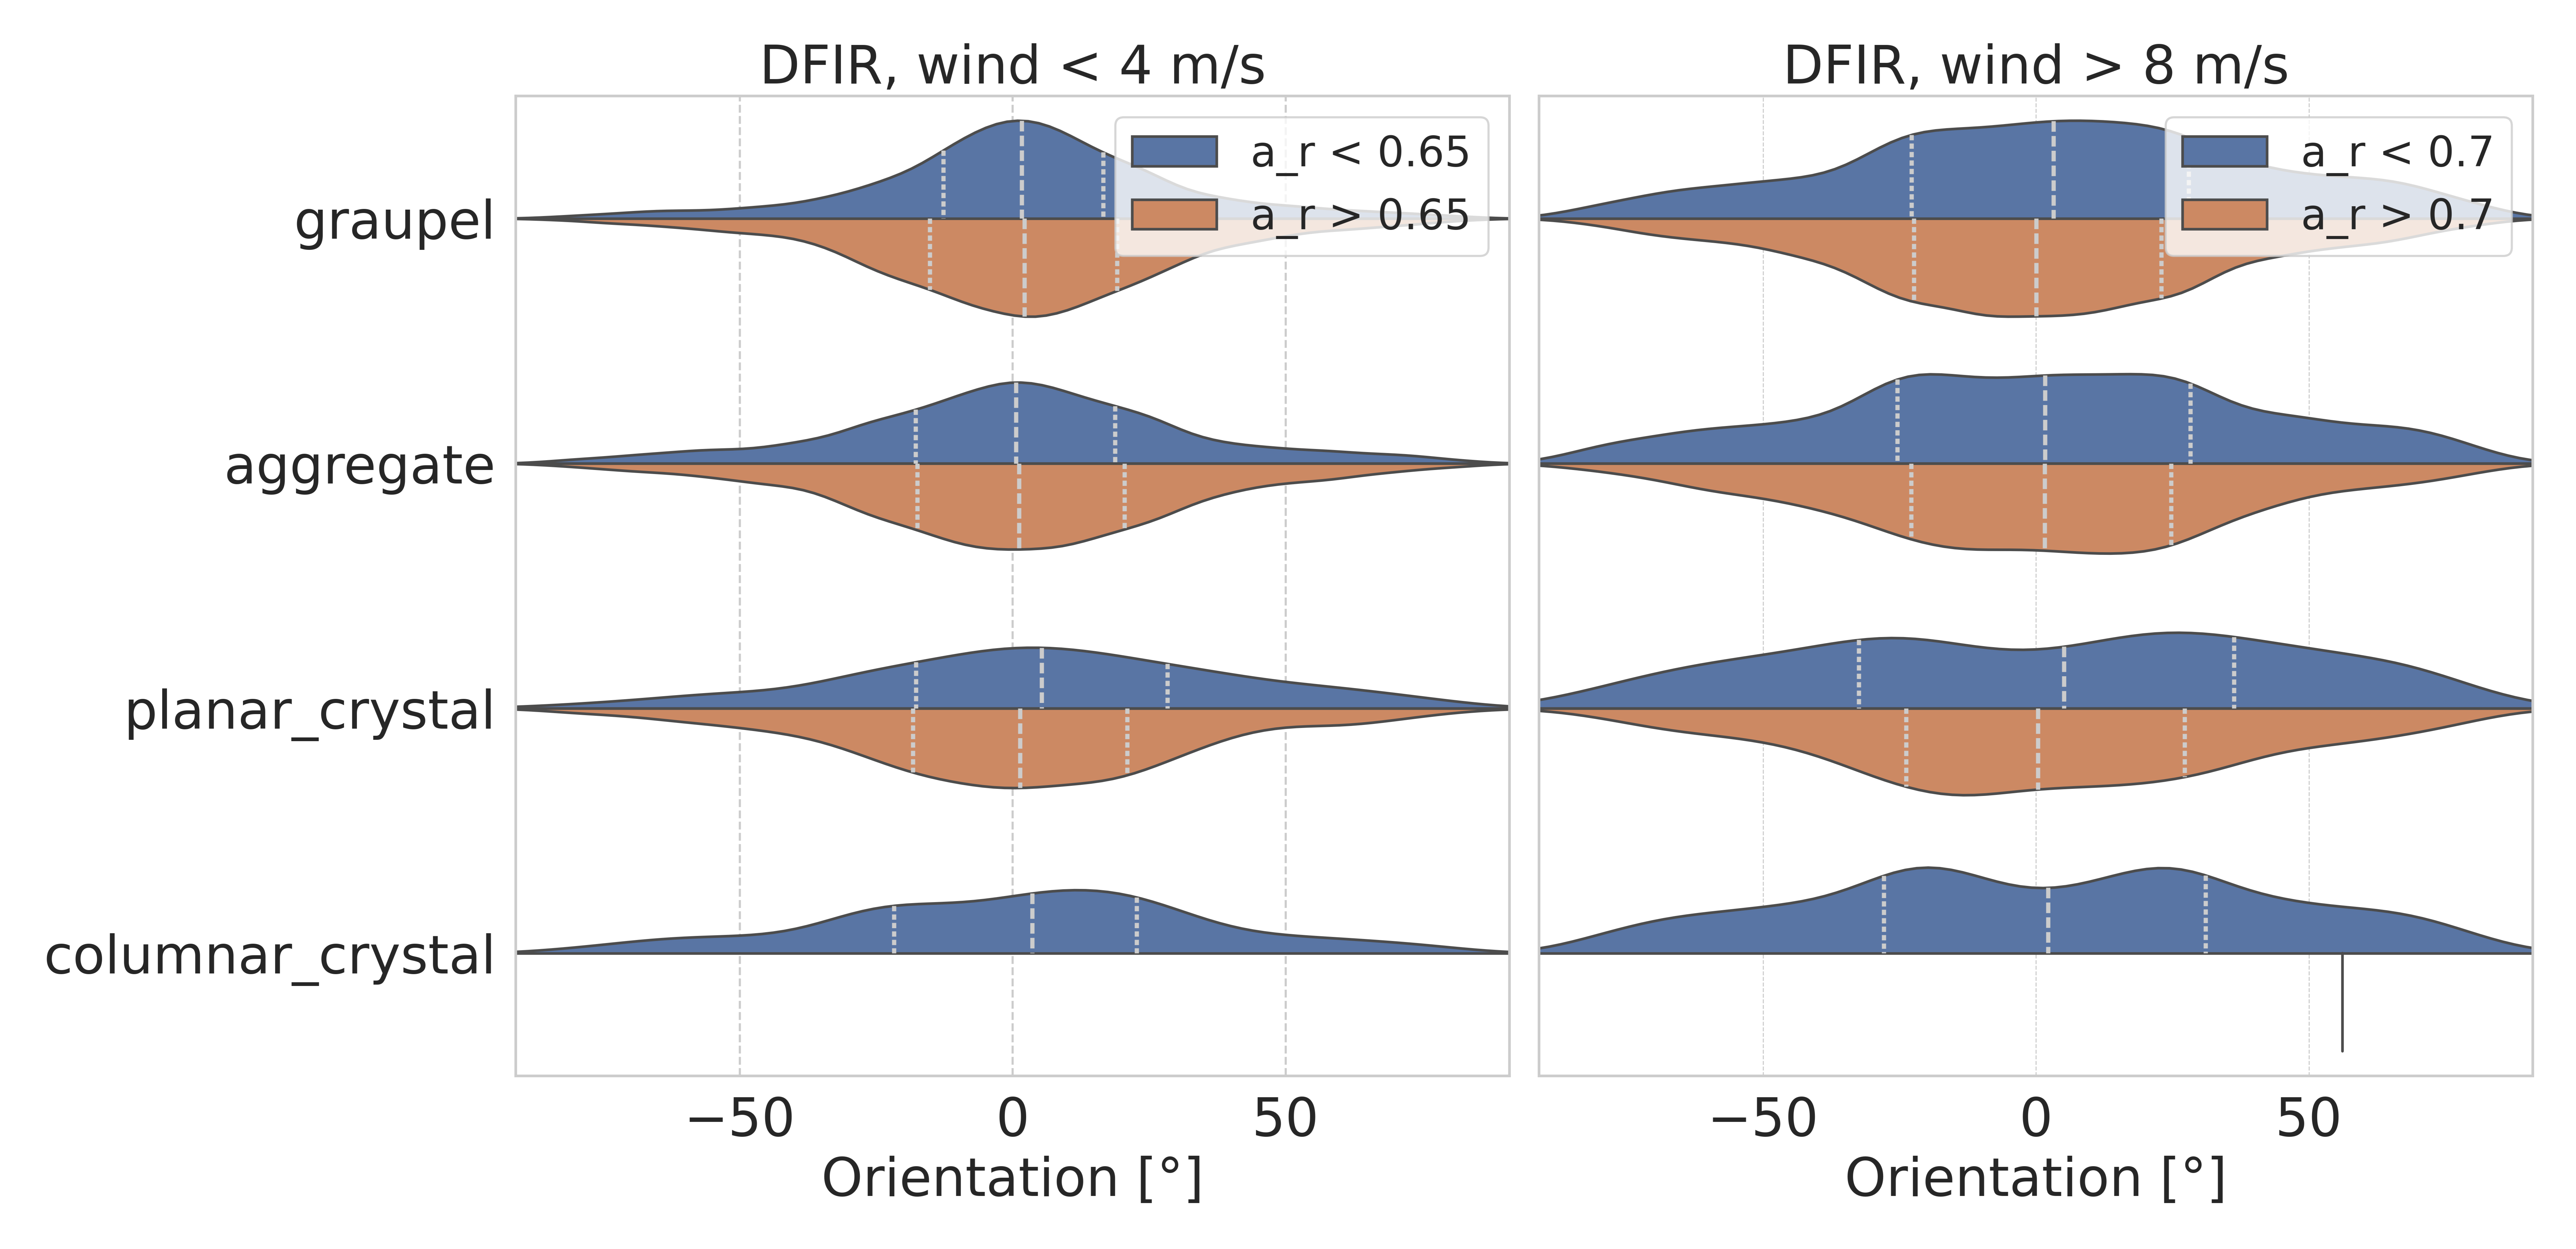
\includegraphics[width=\textwidth]{Fig05.png}
\caption{Violin plot (distribution) of orientation values stratified according to different hydrometeor types. The data correspond to observations collected within a DFIR (Fig.~\ref{fig:wind-effect}), for low horizontal wind (about 47'000 observations for wind $<4$ ms$^{-1}$) and high horizontal wind (about 36'000 observations for wind $>8$ ms$^{-1}$). Data are stratified in two classes of axis ratio (a\_r) limited by the median axis ratio value of the entire population. The number of observations in each distribution ranges between a minimum of 500 (planar crystals, low axis ratio, low wind) and a maximum of about 15'000 (aggregates, low axis ratio, low wind).} 
\label{fig:hydroclass}
\end{figure}



%% SIDEWAYS FIGURE and TABLE
% AGU prefers the use of {sidewaystable} over {landscapetable} as it causes fewer problems.
%
% \begin{sidewaysfigure}
% \includegraphics[width=20pc]{figsamp}
% \caption{caption here}
% \label{newfig}
% \end{sidewaysfigure}
%
%  \begin{sidewaystable}
%  \caption{Caption here}
% \label{tab:signif_gap_clos}
%  \begin{tabular}{ccc}
% one&two&three\\
% four&five&six
%  \end{tabular}
%  \end{sidewaystable}

%% If using numbered lines, please surround equations with \begin{linenomath*}...\end{linenomath*}
%\begin{linenomath*}
%\begin{equation}
%y|{f} \sim g(m, \sigma),
%\end{equation}
%\end{linenomath*}

%%% End of body of article

%%%%%%%%%%%%%%%%%%%%%%%%%%%%%%%%
%% Optional Appendix goes here
%
% The \appendix command resets counters and redefines section heads
%
% After typing \appendix
%
%\section{Here Is Appendix Title}
% will show
% A: Here Is Appendix Title
%
%\appendix
%\section{Here is a sample appendix}

%%%%%%%%%%%%%%%%%%%%%%%%%%%%%%%%%%%%%%%%%%%%%%%%%%%%%%%%%%%%%%%%

%%%%%%%%%%%%%%
% Acronyms
%   \begin{acronyms}
%   \acro{Acronym}
%   Definition here
%   \acro{EMOS}
%   Ensemble model output statistics
%   \acro{ECMWF}
%   Centre for Medium-Range Weather Forecasts
%   \end{acronyms}




\section{Open Research}
The MASCDB dataset used to reproduce the field-based results of this study is openly available in~\citeA{MASCDB_dataset_2023}


%AGU requires an Availability Statement for the underlying data needed to understand, evaluate, and build upon the reported research at the time of peer review and publication.

%Authors should include an Availability Statement for the software that has a significant impact on the research. Details and templates are in the Availability Statement section of the Data and Software for Authors Guidance: \url{https://www.agu.org/Publish-with-AGU/Publish/Author-Resources/Data-and-Software-for-Authors#availability}

%It is important to cite individual datasets in this section and, and they must be included in your bibliography. Please use the type field in your bibtex file to specify the type of data cited. Some options include Dataset, Software, Collection, ComputationalNotebook. Ex: 

\acknowledgments



%% ------------------------------------------------------------------------ %%
%% References and Citations

%%%%%%%%%%%%%%%%%%%%%%%%%%%%%%%%%%%%%%%%%%%%%%%
%
\bibliography{references,references_data}
%
% don't specify bibliographystyle

% In the References section, cite the data/software described in the Availability Statement (this includes primary and processed data used for your research). For details on data/software citation as well as examples, see the Data & Software Citation section of the Data & Software for Authors guidance
% https://www.agu.org/Publish-with-AGU/Publish/Author-Resources/Data-and-Software-for-Authors#citation

%%%%%%%%%%%%%%%%%%%%%%%%%%%%%%%%%%%%%%%%%%%%%%%

%\bibliography{enter your bibtex bibliography filename here}



%Reference citation instructions and examples:
%
% Please use ONLY \cite and \citeA for reference citations.
% \cite for parenthetical references
% ...as shown in recent studies (Simpson et al., 2019)
% \citeA for in-text citations
% ...Simpson et al. (2019) have shown...
%
%
%...as shown by \citeA{jskilby}.
%...as shown by \citeA{lewin76}, \citeA{carson86}, \citeA{bartoldy02}, and \citeA{rinaldi03}.
%...has been shown \cite{jskilbye}.
%...has been shown \cite{lewin76,carson86,bartoldy02,rinaldi03}.
%... \cite <i.e.>[]{lewin76,carson86,bartoldy02,rinaldi03}.
%...has been shown by \cite <e.g.,>[and others]{lewin76}.
%
% apacite uses < > for prenotes and [ ] for postnotes
% DO NOT use other cite commands (e.g., \citet, \citep, \citeyear, \citealp, etc.).
% \nocite is okay to use to add references from your Supporting Information
%



\end{document}



More Information and Advice:

%% ------------------------------------------------------------------------ %%
